\documentclass{beamer}
\usetheme{Madrid}

\usepackage[italian]{babel}

\usepackage[utf8]{inputenc}

\usepackage{hyperref}

\usepackage{graphicx}
\graphicspath{{images/}}

\usepackage{geometry}
\geometry{mag=2500,truedimen}

\usepackage{tcolorbox}
\tcbuselibrary{minted,breakable}
\newtcblisting{myvhdl}[1]{%
  listing only,
  minted language=vhdl,
  minted options={breaklines,fontsize=\tiny},
  fonttitle=\tiny \bfseries,
  breakable,
  boxsep=0.5mm,
  left=0.5mm,
  right=0.5mm,
  top=0.5mm,
  bottom=0.5mm,
  title=#1
}
\newcommand{\BashFancyFormatLine}{%
  \def\FancyVerbFormatLine##1{\$\,##1}%
}
\newtcblisting{commandshell}{%
  colback=black,
  colupper=white,
  breakable,
  colframe=yellow!75!black,
  listing only,
  boxsep=0.5mm,
  left=0.5mm,
  right=0.5mm,
  top=0.5mm,
  bottom=0.5mm,
  minted options={fontsize=\tiny,breaklines,formatcom=\BashFancyFormatLine}}
\newtcblisting{basetcblisting}{%
  listing only,
  breakable,
  boxsep=0.5mm,
  left=0.5mm,
  right=0.5mm,
  top=0.5mm,
  bottom=0.5mm,
}

\usepackage{courier}

\usepackage{listings}
\lstset{
  basicstyle=\ttfamily,
  breaklines=true
}

\title{Il Processore Mic-1}
\subtitle{Implementazione}
\author[Architettura dei Sistemi di Elaborazione]{Prof.\ Nicola Mazzocca\\
  Ing. Alberto Moriconi}
\institute[]{Corso di Architettura dei Sistemi di Elaborazione\\
  Università degli Studi di Napoli Federico II}
\date{}

\begin{document}
\begin{frame}
\titlepage{}
\end{frame}

\section{Introduzione}
\begin{frame}[fragile]
  \frametitle{Macchine a Stack}
  Il processore Mic-1 è una macchina \textit{a stack}, e non dispone di registri generali.
  \begin{columns}
    \begin{column}{0.5\textwidth}
      Consideriamo l'istruzione Java:
      \begin{basetcblisting}
  a1 = a2 + a3;\end{basetcblisting}
    \end{column}
    \begin{column}{0.5\textwidth}
      In assembly IJVM, è tradotta come:
      \begin{basetcblisting}
  ILOAD a2    (a)
  ILOAD a3    (b)
  IADD        (c)
  ISTORE a1   (d)\end{basetcblisting}
    \end{column}
  \end{columns}
  Osserviamo come evolve lo stack:
  \begin{center}
    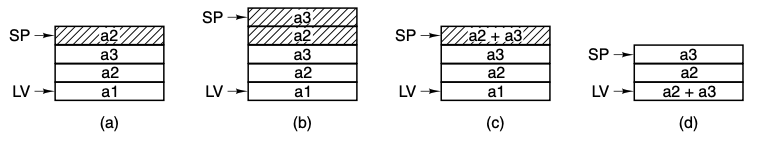
\includegraphics[width=\textwidth]{stack_add.png}
  \end{center}
\end{frame}

\section{Unità Operativa}
\begin{frame}[fragile]
  \frametitle{Unità Operativa}
  \begin{columns}
    \begin{column}{0.4\textwidth}
      \begin{center}
        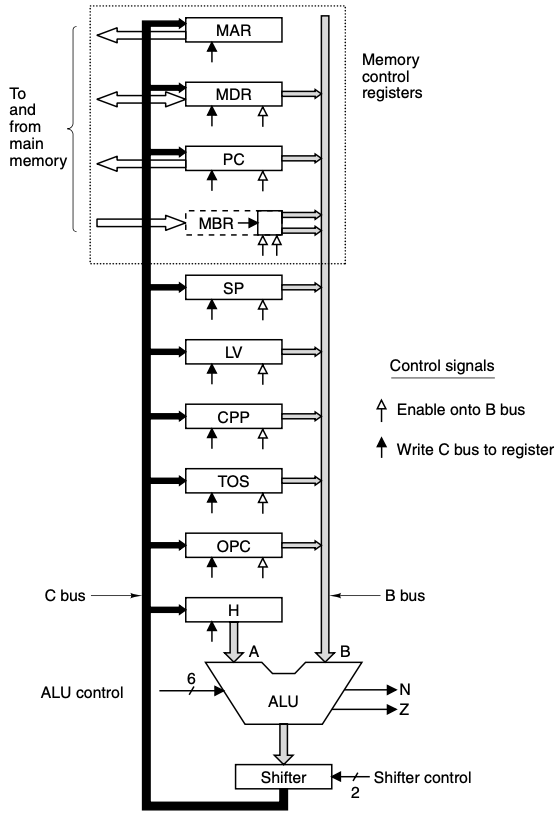
\includegraphics[width=\textwidth]{datapath.png}
      \end{center}
    \end{column}
    \begin{column}{0.6\textwidth}
      \begin{myvhdl}{datapath.vhd}
entity datapath is
  port (
    clk              : in  std_logic;
    reset            : in  std_logic;
    alu_control      : in  alu_ctrl_type;
    c_to_reg_control : in  c_ctrl_type;
    mem_control      : in  mem_ctrl_type;
    reg_to_b_control : in  b_ctrl_type;
    mbr_reg_out      : out mbr_data_type;
    alu_n_flag       : out std_logic;
    alu_z_flag       : out std_logic;
    mem_data_we      : out std_logic;
    mem_data_in      : in  reg_data_type;
    mem_data_out     : out reg_data_type;
    mem_data_addr    : out reg_data_type;
    mem_instr_in     : in  mbr_data_type;
    mem_instr_addr   : out reg_data_type
    );
end entity datapath;

architecture behavioral of datapath is
  -- Come la implementiamo?
end architecture behavioral;
\end{myvhdl}
    \end{column}
  \end{columns}
\end{frame}

\begin{frame}[fragile]
  \frametitle{Componenti}
  \begin{columns}
    \begin{column}{0.4\textwidth}
      \begin{center}
        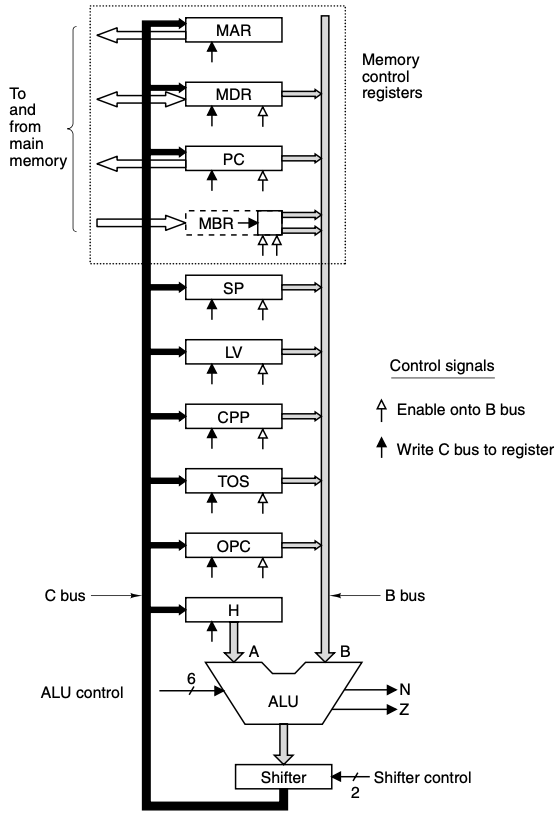
\includegraphics[width=\textwidth]{datapath.png}
      \end{center}
    \end{column}
    \begin{column}{0.6\textwidth}
      Per implementare l'unità operativa dobbiamo scrivere in VHDL il codice
      relativo:
      \begin{itemize}
        \item ai registri;
        \item all'ALU;
        \item ai bus.
      \end{itemize}
    \end{column}
  \end{columns}
\end{frame}

\begin{frame}[fragile]
  \frametitle{Registri} I registri sono implementati con un singolo
  \lstinline{process}, che ne gestisce la logica di reset e quella di scrittura
  mediante il bus \lstinline{C}:

  \begin{columns}
    \begin{column}{0.45\textwidth}
      \begin{myvhdl}{datapath.vhd}
-- Registers
signal sp_reg  : reg_data_type;
signal lv_reg  : reg_data_type;
signal cpp_reg : reg_data_type;
[...]
\end{myvhdl}

\begin{myvhdl}{common\_defs.vhd}
--! Processor register data width
constant reg_data_width : positive := 32;
[...]
--! Processor register data
subtype reg_data_type is
  std_logic_vector(reg_data_width - 1 downto 0);
[...]
--! C control MAR bit
constant c_ctrl_mar : natural := 0;
--! C control MDR bit
constant c_ctrl_mdr : natural := 1;
[...]
\end{myvhdl}
\end{column}

\begin{column}{0.55\textwidth}
  \begin{myvhdl}{datapath.vhd}
-- Processor registers
reg_proc : process(clk) is
begin
  if rising_edge(clk) then
    if reset = '1' then
      mar_reg <= (others => '0');
      pc_reg  <= (others => '0');
      [...]
    else
      if c_to_reg_control(c_ctrl_mar) = '1' then
        mar_reg <= c_bus;
      end if;
      if c_to_reg_control(c_ctrl_pc) = '1' then
        pc_reg <= c_bus;
      end if;
      [...]
    end if;
  end if;
end process reg_proc;
\end{myvhdl}
    \end{column}
  \end{columns}
\end{frame}

\begin{frame}
  \frametitle{Convenzioni sui Registri}
  \begin{columns}
    \begin{column}{0.5\textwidth}
  Alcuni registri sono cablati in modo da poter essere usati solo per uno scopo
  specifico:
  \begin{itemize}
    \item i registri dell'interfaccia con la memoria:
    \begin{itemize}
      \item \lstinline{MAR} - memory address register;
      \item \lstinline{MDR} - memory data register;
      \item \lstinline{PC} - program counter;
      \item \lstinline{MBR} - memory byte register;
    \end{itemize}
    \item il registro che mantiene il primo operando dell'ALU:
    \begin{itemize}
      \item \lstinline{H} - holding.
    \end{itemize}
  \end{itemize}
  \end{column}

  \begin{column}{0.5\textwidth}
    Gli altri registri sono funzionalmente equivalenti, ed i loro nomi sono
    assegnati sulla base dell'uso che se ne fa nel microprogramma:
  \begin{itemize}
    \item \lstinline{SP} - stack pointer;
    \item \lstinline{LV} - local variables;
    \item \lstinline{CPP} - constant pool pointer;
    \item \lstinline{TOS} - top of stack;
    \item \lstinline{OPC} - scratch register.
  \end{itemize}
\end{column}
\end{columns}
\end{frame}

\begin{frame}[fragile]
  \frametitle{ALU}
  L'implementazione dell'ALU è puramente behavioral:
  \begin{columns}
    \begin{column}{0.5\textwidth}
  \begin{myvhdl}{alu.vhd}
entity alu is
  port (
    --! ALU control
    control       : in  alu_ctrl_type;
    --! ALU operand A
    operand_a     : in  reg_data_type;
    --! ALU operand B
    operand_b     : in  reg_data_type;
    --! ALU result
    sh_result     : out reg_data_type;
    --! Negative flag
    negative_flag : out std_logic;
    --! Zero flag
    zero_flag     : out std_logic
    );
end entity alu;

architecture behavioral of alu is
  [...]
end architecture behavioral;
\end{myvhdl}
\end{column}
\begin{column}{0.5\textwidth}
\begin{center}
  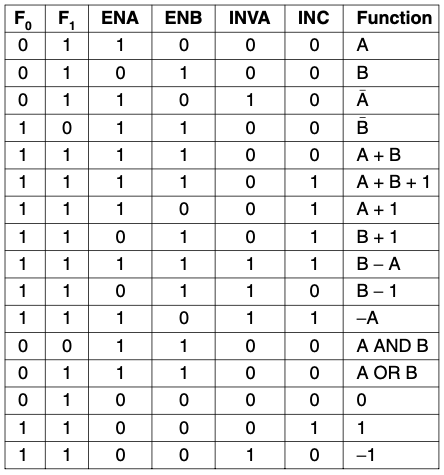
\includegraphics[width=\textwidth]{alu_func.png}
\end{center}
\end{column}
\end{columns}
\end{frame}

\begin{frame}[fragile]
  \frametitle{Bus}
  \begin{columns}
    \begin{column}{0.5\textwidth}
      A ciascun bus corrisponde un \lstinline{signal} VHDL:
\begin{myvhdl}{datapath.vhd}
signal a_bus : reg_data_type;
signal b_bus : reg_data_type;
signal c_bus : reg_data_type;
\end{myvhdl}
    \end{column}
    \begin{column}{0.5\textwidth}
      Il multiplexer che disciplina l'accesso al bus \lstinline{B} è
      implementato utilizzando il costrutto \lstinline{with/select}:
      \begin{myvhdl}{datapath.vhd}
with reg_to_b_control select b_bus <=
  mdr_reg         when b_ctrl_mdr,
  pc_reg          when b_ctrl_pc,
  mbr_s           when b_ctrl_mbr,
  mbr_u           when b_ctrl_mbru,
  sp_reg          when b_ctrl_sp,
  lv_reg          when b_ctrl_lv,
  cpp_reg         when b_ctrl_cpp,
  tos_reg         when b_ctrl_tos,
  opc_reg         when b_ctrl_opc,
  (others => '0') when others;
\end{myvhdl}
\end{column}
\end{columns}

\begin{block}{Logica tri-state}
  In altri corsi è presentato anche un altro modo di disciplinare l'accesso ai
  bus: facendo uso di buffer tri-state. Gli FPGA che utilizziamo non dispongono
  però di buffer tri-state se non ai pad di IO.
\end{block}
\end{frame}

\begin{frame}
  \frametitle{Ricapitolando}
  \begin{columns}
    \begin{column}{0.4\textwidth}
      \begin{center}
        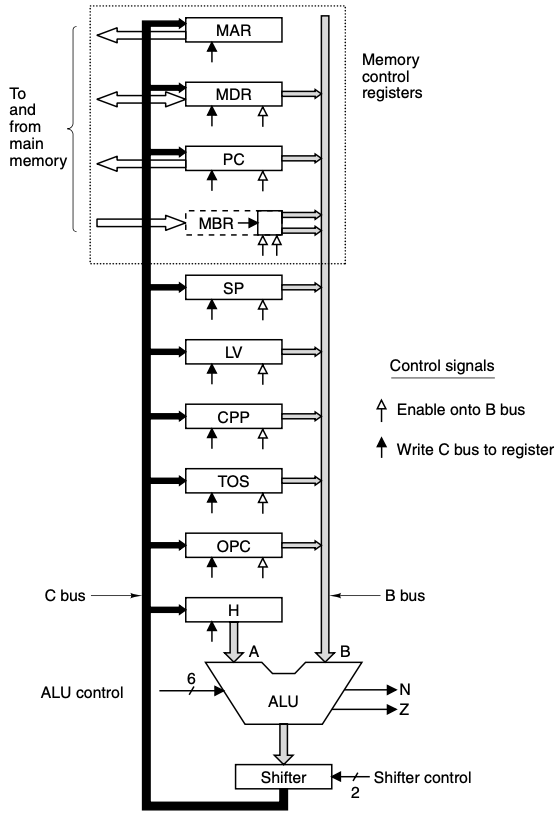
\includegraphics[width=\textwidth]{datapath.png}
      \end{center}
    \end{column}
    \begin{column}{0.6\textwidth}
  Abbiamo implementato:
  \begin{itemize}
    \item i registri con un \lstinline{process};
    \item l'ALU con un \lstinline{component} con architettura behavioral;
    \item la disciplina di accesso al bus \lstinline{B} con un costrutto
    \lstinline{with/select}.
  \end{itemize}
  Queste parti evolvono \textbf{concorrentemente}.
\end{column}
\end{columns}
\end{frame}

\begin{frame} [fragile]
  \frametitle{Protocollo con la Memoria}
  \begin{center}
    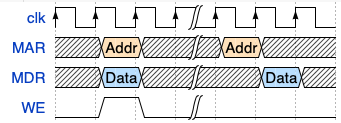
\includegraphics[width=0.4\textwidth]{mem_prot.png}
  \end{center}
  Consideriamo l'interfaccia dati \lstinline{MAR}/\lstinline{MDR} (indirizzo e dato su 32 bit):
  \begin{itemize}
    \item Per eseguire una scrittura, l'indirizzo e il dato devono essere
    disponibili nei registri \lstinline{MAR} e \lstinline{MDR} al fronte di
    salita in cui è alto il segnale \lstinline{WE}.
    \item Quando si opera in lettura (\lstinline{WE} basso), il dato è
    disponibile nel registro \lstinline{MDR} al fronte di clock successivo
    rispetto a quello in cui l'indirizzo è posto nel registro \lstinline{MAR}.
  \end{itemize}
\end{frame}

\begin{frame}[fragile]
  \frametitle{Protocollo con la Memoria (2)}
  \begin{columns}
    \begin{column}{0.5\textwidth}
      La lettura e la generazione del segnale di \textit{write enable} sono
      implementate in un \lstinline{process}:
      \begin{myvhdl}{datapath.vhd}
-- Processor registers
reg_proc : process(clk) is
begin
  [...]
  if c_to_reg_control(c_ctrl_mdr) = '1' then
    mdr_reg <= c_bus;
  elsif rd_ff = '1' then
    mdr_reg <= mem_data_in;
  end if;
  [...]
  wr_ff <= mem_control(mem_ctrl_write);
end process;
\end{myvhdl}
\end{column}
\begin{column}{0.5\textwidth}
  I registri dell'interfaccia e il segnale di \textit{write enable} sono
  assegnati alle uscite dell'\lstinline{entity}:
  \begin{myvhdl}{datapath.vhd}
-- Output
mem_data_out  <= mdr_reg;
mem_data_addr <= mar_reg;
mem_data_we   <= wr_ff;
\end{myvhdl}
\end{column}
\end{columns}
\begin{block}{Interfaccia istruzioni}
  L'interfaccia istruzioni \lstinline{PC}/\lstinline{MBR} (indirizzo su 32 bit,
  dato su 8 bit) opera in modo simile in lettura, e non prevede operazioni di
  scrittura.
\end{block}
\end{frame}

\section{Microistruzioni}
\begin{frame}
  \frametitle{Segnali di Controllo}
  Per controllare l'unità operativa sono necessari:
  \begin{itemize}
    \item 9 segnali per controllare la scrittura dei dati dal bus \lstinline{C}
    ai registri;
    \item 4 segnali per controllare quale registro è collegato al bus
    \lstinline{B} e va in ingresso all'ALU;
    \item 8 segnali per controllare l'ALU;
    \item 2 segnali per abilitare lettura/scrittura sull'interfaccia
    \lstinline{MAR}/\lstinline{MDR};
    \item 1 segnale per abilitare il fetch sull'interfaccia
    \lstinline{PC}/\lstinline{MBR}.
  \end{itemize}
  Inoltre ogni microistruzione deve contenere dei bit aggiuntivi per indicare la
  microistruzione successiva e per il controllo di flusso.
\end{frame}

\begin{frame}
  \frametitle{Formato delle Microistruzioni}
  \begin{center}
    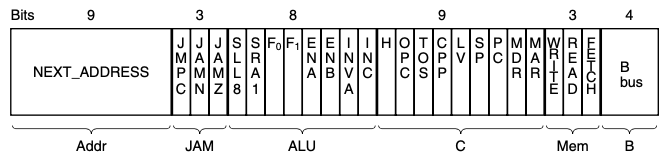
\includegraphics[width=0.8\textwidth]{mu_instr_small.png}
  \end{center}
\begin{itemize}
  \item \lstinline{Addr} - Indirizzo di una potenziale prossima microistruzione;
  \item \lstinline{JAM} - Determina come è selezionata la prossima
  microistruzione;
  \item \lstinline{ALU} - Controllo dell'ALU e dello shifter;
  \item \lstinline{C} - Controlla quali registri vengono scritti dal bus
  \lstinline{C};
  \item \lstinline{Mem} - Controlla le operazioni di memoria;
  \item \lstinline{B} - Seleziona il registro connesso al bus \lstinline{B}.
\end{itemize}
\end{frame}

\begin{frame}
  \frametitle{Esempio: l'istruzione \lstinline{IADD}}
  Trascurando per ora i campi \lstinline{Addr} e \lstinline{JAM}, siamo in grado
di codificare gli altri campi delle microistruzioni:
\begin{enumerate}
  \item
  \begin{itemize}
    \item \lstinline{ALU}: \lstinline{110110} (decremento dell'operando \lstinline{B});
    \item \lstinline{C}: \lstinline{000001001} (bus \lstinline{C} scrive su
    \lstinline{SP} e \lstinline{MAR});
    \item \lstinline{Mem}: \lstinline{010} (lettura dati);
    \item \lstinline{B}: \lstinline{0100} (\lstinline{SP} controlla il bus \lstinline{B}).
  \end{itemize}
  \item
  \begin{itemize}
    \item \lstinline{ALU}: \lstinline{010100} (l'operando \lstinline{B} passa invariato);
    \item \lstinline{C}: \lstinline{100000000} (bus \lstinline{C} scrive su
    \lstinline{H});
    \item \lstinline{Mem}: \lstinline{000} (nessuna operazione di memoria);
    \item \lstinline{B}: \lstinline{0111} (\lstinline{TOS} controlla il bus \lstinline{B}).
  \end{itemize}
  \item
  \begin{itemize}
    \item \lstinline{ALU}: \lstinline{111100} (somma degli operandi
    \lstinline{A} e \lstinline{B});
    \item \lstinline{C}: \lstinline{001000010} (bus \lstinline{C} scrive su
    \lstinline{MDR} e \lstinline{TOS});
    \item \lstinline{Mem}: \lstinline{100} (scrittura dati);
    \item \lstinline{B}: \lstinline{0000} (\lstinline{MDR} controlla il bus \lstinline{B}).
  \end{itemize}
\end{enumerate}
\end{frame}

\section{Unità di Controllo}
\begin{frame}
  \frametitle{Unità di Controllo}
  \begin{columns}
    \begin{column}{0.6\textwidth}
      \begin{center}
        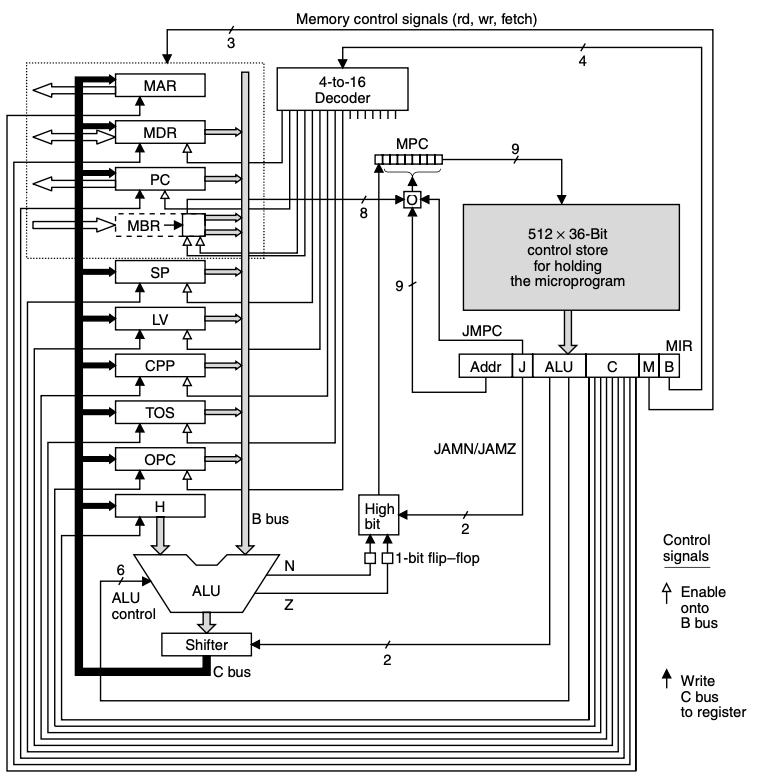
\includegraphics[width=\textwidth]{mic1.png}
      \end{center}
    \end{column}
    \begin{column}{0.4\textwidth}
      L'unità di controllo del Mic-1 si comporta come un \textit{sequencer},
      producendo in ciascun ciclo:
\begin{enumerate}
  \item lo stato dei segnali di controllo;
  \item l'indirizzo della prossima microistruzione da eseguire.
\end{enumerate}
    \end{column}
  \end{columns}
\end{frame}

\begin{frame}[fragile]
  \frametitle{Control Store}
  Le microistruzioni sono memorizzate in una ROM interna all'unità di controllo,
  denominata \textit{control store}:
  \begin{columns}
    \begin{column}{0.5\textwidth}
\begin{myvhdl}{control\_store.vhd}
entity control_store is
  port (
    --! Address of the desired word
    address : in  ctrl_str_addr_type;
    --! Content of the addressed word
    word    : out ctrl_str_word_type
    );
end entity control_store;
\end{myvhdl}
\end{column}
\begin{column}{0.5\textwidth}
\begin{myvhdl}{control\_store.vhd}
constant words : ctrl_str_type := (
--BEGIN_WORDS_ENTRY
0 => "000000110000000000000000000000001001",
1 => "010111100000000000000000000000001001",
2 => "000000000000000000000000000000000000",
[...]
--END_WORDS_ENTRY
);
\end{myvhdl}
\end{column}
\end{columns}
\begin{myvhdl}{common\_defs.vhd}
--! Control store address
subtype ctrl_str_addr_type is std_logic_vector(ctrl_str_addr_width - 1 downto 0);
--! Control store word
subtype ctrl_str_word_type is std_logic_vector(ctrl_str_word_width - 1 downto 0);
[...]
--! Control store word
subtype ctrl_str_word_type is std_logic_vector(ctrl_str_word_width - 1 downto 0);
[...]
--! Control store content
type ctrl_str_type is array (ctrl_str_words - 1 downto 0) of ctrl_str_word_type;
\end{myvhdl}
\end{frame}

\begin{frame}[fragile]
  \frametitle{Altra Logica di Controllo}
  Inoltre, l'unità di controllo contiene:
  \begin{itemize}
    \item i registri \lstinline{MIR} e \lstinline{MPC} di interfaccia con il
    control store;
    \item il decoder per i segnali di controllo del bus \lstinline{B};
    \item la logica per determinare l'indirizzo della prossima microistruzione.
  \end{itemize}
  A livello microprogramma, i salti sono controllati mediante il campo
  \lstinline{JAM}: i due bit \lstinline{JAMN} e \lstinline{JAMZ}
  sono combinati con i valori dei flag \lstinline{N} e \lstinline{Z} dell'ALU, e
  permettono di modificare il bit più significativo dell'\lstinline{MPC}:

\begin{lstlisting}
  MPC[8] = (JAMZ AND Z) OR (JAMN AND N) OR Addr[8]
\end{lstlisting}

  Se il bit \lstinline{JMPC} è asserito, gli 8 bit meno significativi di
  \lstinline{MPC} sono messi in \lstinline{OR} bit-a-bit con gli 8 bit contenuti
  nel registro \lstinline{MBR}:

\begin{lstlisting}
  MPC[7:0] = Addr[7:0] OR (MBR[7:0] AND JMPC)
\end{lstlisting}
\end{frame}

\begin{frame}[fragile]
  \frametitle{Altra Logica di Controllo (2)}
  Il decoder è implementato con un \lstinline{process}:
  \begin{myvhdl}{control\_unit.vhd}
-- B_BUS control decoder
reg_to_b_decoder : process(mir_reg(ctrl_b'range)) is
begin
  reg_to_b_decoder_out <= (others => '0');

  if unsigned(mir_reg(ctrl_b'range)) < b_ctrl_width then
    reg_to_b_decoder_out(to_integer(unsigned(mir_reg(ctrl_b'range)))) <= '1';
  end if;
end process reg_to_b_decoder;
\end{myvhdl}
La logica di salto è implementata con delle assegnazioni su un \textit{virtual
  register}, i.e. dei semplici \lstinline{signal} che rimangono stabili fino al
fronte di clock successivo:
\begin{myvhdl}{control\_unit.vhd}
-- MPC virtual register
ctrl_nxt_addr_no_msb <= mir_reg(ctrl_nxt_addr_no_msb_type'range);
jmpc_addr <= ctrl_nxt_addr_no_msb or mbr_reg_in
             when mir_reg(ctrl_jmpc) = '1'
             else ctrl_nxt_addr_no_msb;
high_bit <= (alu_n_flag and mir_reg(ctrl_jamn))
            or (alu_z_flag and mir_reg(ctrl_jamz));
mpc_virtual_reg <= (mir_reg(ctrl_nxt_addr_msb) or high_bit) & jmpc_addr;
\end{myvhdl}
\end{frame}

\begin{frame}[fragile]
  \frametitle{Sequencing delle Microistruzioni}
  L'unità di controllo si comporta effettivamente come un \textit{sequencer}.
  \begin{columns}
    \begin{column}{0.5\textwidth}
\begin{myvhdl}{ajvm.mal}
main:
    PC = PC + 1; fetch; goto (MBR)
\end{myvhdl}
\end{column}
\begin{column}{0.5\textwidth}
\begin{myvhdl}{ajvm.mal}
iadd = 0x65:
    MAR = SP = SP - 1; rd
    H = TOS
    MDR = TOS = MDR + H; wr; goto main
\end{myvhdl}
\end{column}
\end{columns}
\begin{enumerate}
  \item Dopo una fase di inizializazione, viene eseguita la microistruzione
  \lstinline{main} che incrementa il \lstinline{PC}, esegue il fetch di
  un'istruzione e imposta come prossima microistruzione quella ``puntata'' dal
  registro \lstinline{MBR}.
  \item Se ad esempio l'istruzione prelevata su \lstinline{MBR} è
  \lstinline{0x65}, viene eseguita la microistruzione all'indirizzo
  \lstinline{0x65} del control store, la \lstinline{IADD}.
  \item Dopo le tre microistruzioni della \lstinline{IADD} viene rieseguita la
  microistruzione alla label \lstinline{main}, che esegue il fetch della
  prossima istruzione.
\end{enumerate}
\end{frame}

\begin{frame}[fragile]
  \frametitle{Esempi di Istruzioni IJVM}
  \begin{columns}
    \begin{column}{0.5\textwidth}
      Esempi di codici di movimento:
\begin{myvhdl}{ajvm.mal}
iload = 0x15:
        H = LV
        MAR = MBRU + H; rd
iload_cont:
        MAR = SP = SP + 1
        PC = PC + 1; fetch; wr
        TOS = MDR; goto main

istore = 0x36:
        H = LV
        MAR = MBRU + H
istore_cont:
        MDR = TOS; wr
        SP = MAR = SP - 1; rd
        PC = PC + 1; fetch
        TOS = MDR; goto main
\end{myvhdl}
\end{column}
\begin{column}{0.5\textwidth}
  Esempi di codici di salto:
\begin{myvhdl}{ajvm.mal}
ijvm_goto = 0xA7:
        OPC = PC - 1
goto_cont:
        PC = PC + 1; fetch
        H = MBR << 8
        H = MBRU OR H
        PC = OPC + H; fetch
        goto main

[...]

ifeq = 0x99:
        MAR = SP = SP - 1; rd
        OPC = TOS
        TOS = MDR
        Z = OPC; if (Z) goto T; else goto F

[...]

T:
        OPC = PC - 1; fetch; goto goto_cont

F:
        PC = PC + 1
        PC = PC + 1; fetch
        goto main
\end{myvhdl}
    \end{column}
    \end{columns}
\end{frame}

\begin{frame}
  \frametitle{Esempi di Istruzioni IJVM (2)}
  Consideriamo l'istruzione \lstinline{ILOAD varnum}, con \lstinline{varnum}
  variabile da caricare su stack (offset rispetto al puntatore in
  \lstinline{LV}), codificata su 1 byte:
  \begin{enumerate}
    \item il puntatore contenuto in \lstinline{LV} è scritto in \lstinline{H};
    \item in \lstinline{MAR} è posta la somma base \lstinline{LV} + offset
    \lstinline{MBRU}, e si abilita la lettura;
    \begin{itemize}
      \item \lstinline{MBRU} significa: contenuto di \lstinline{MBR}, come
      unsigned;
      \item il contenuto di \lstinline{MBR} è il risultato dell'ultimo
      \lstinline{fetch} eseguito dalla microistruzione \lstinline{main};
    \end{itemize}
    \item \lstinline{MAR} e \lstinline{SP} sono posti ad una nuova posizione
    vuota su stack (dove sarà fatto il push del nuovo elemento); inoltre il dato
    di cui eseguire il push è ora disponibile in \lstinline{MDR};
    \item \lstinline{PC} è incrementato e si fa il \lstinline{fetch} della
    prossima istruzione (in modo che \lstinline{main} possa eseguire il
    \lstinline{goto} alla microistruzione corretta); si esegue anche la
    scrittura (push) in memoria;
    \item il contenuto di \lstinline{TOS} è aggiornato con il dato di cui si è
    eseguito il push.
  \end{enumerate}
\end{frame}
 
\section{Toolchain}
\begin{frame}[fragile]
  \frametitle{Installazione dei Tool}
  In caso di dubbi, fare riferimento alle dispense per la procedura dettagliata.
\begin{commandshell}
sudo apt install git gradle cmake ghdl gtkwave
mkdir esercitazione_mic
cd esercitazione_mic
mkdir tools
git clone https://github.com/albmoriconi/mal.git
cd mal
./gradlew build
cd ..
git clone https://github.com/albmoriconi/ajvm.git
cd ajvm
./gradlew build
cd ..
tar -xvf mal/build/distributions/mal.tar -C tools/
tar -xvf ajvm/build/distributions/ajvm.tar -C tools/
git clone https://github.com/albmoriconi/amic-0.git
cd amic-0
mkdir build
cd build
cmake ..
\end{commandshell}
\end{frame}

\begin{frame}
  \frametitle{Struttura del Progetto}
  La directory principale del repository amic-0 è organizzata come segue:
\begin{itemize}
  \item \lstinline{src} - codice sorgente
  \begin{itemize}
    \item \lstinline{main} - implementazione (subdirectory ordinate per
    linguaggio)
    \item \lstinline{test} - testbench (subdirectory ordinate per linguaggio)
  \end{itemize}
  \item \lstinline{util} - utility necessarie per il flow di sviluppo
  (subdirectory ordinate per linguaggio)
  \item \lstinline{build} - contiene i file prodotti dal build system (questa
  directory deve essere creata manualmente)
\end{itemize}

Ogni directory che contiene codice (eventualmente nelle subdirectory) contiene
anche un file \lstinline{CMakeLists.txt} che serve al build system per tenere
traccia dei sorgenti e aggiungerli ai target opportuni.
\end{frame}

\begin{frame}
  \frametitle{Flow di Sviluppo}
  \begin{enumerate}
    \item Per modificare microprogramma e programma bisogna modificarne i file e
    lanciare i target make relativi.
  \begin{itemize}
    \item \lstinline{src/main/mal/ajvm.mal} - microprogramma
    \begin{itemize}
      \item \lstinline{make create_control_store}
    \end{itemize}
    \item \lstinline{src/main/ajvm/program.ajvm} - programma
    \begin{itemize}
      \item \lstinline{make create_ram}
    \end{itemize}
  \end{itemize}
  \item Per lanciare la suite di test va lanciato il target \lstinline{make
    check}
  \item Le forme d'onda (visualizzabili con \lstinline{gtkwave}) sono salvate
  nella directory \lstinline{build/src/test/vhdl}.
\end{enumerate}
Per aggiungere altri testbench alla suite:
\begin{enumerate}
  \item salvarli nella directory \lstinline{test/vhdl};
  \item modificare il file \lstinline{test/vhdl/CmakeLists.txt} aggiungendo alla
  macro \lstinline{add_vhdl_test_sources} un'entry relativa al nuovo testbench.
\end{enumerate}
\end{frame}

\begin{frame}
  \frametitle{Risultati dei Test (Esempio)}
  \begin{center}
    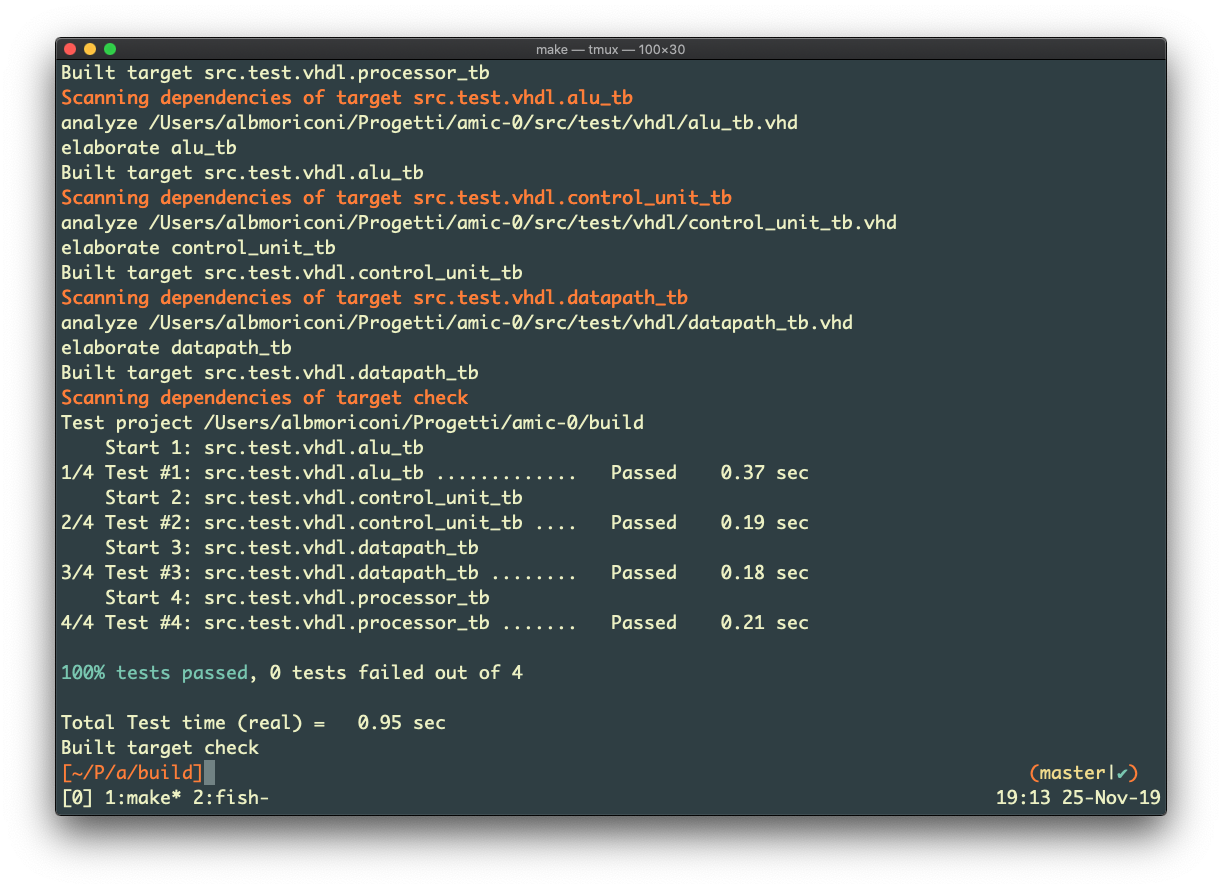
\includegraphics[width=0.9\textwidth]{test.png}
  \end{center}
\end{frame}

\begin{frame}
  \frametitle{Waveform dei Testbench (Esempio)}
  \begin{center}
    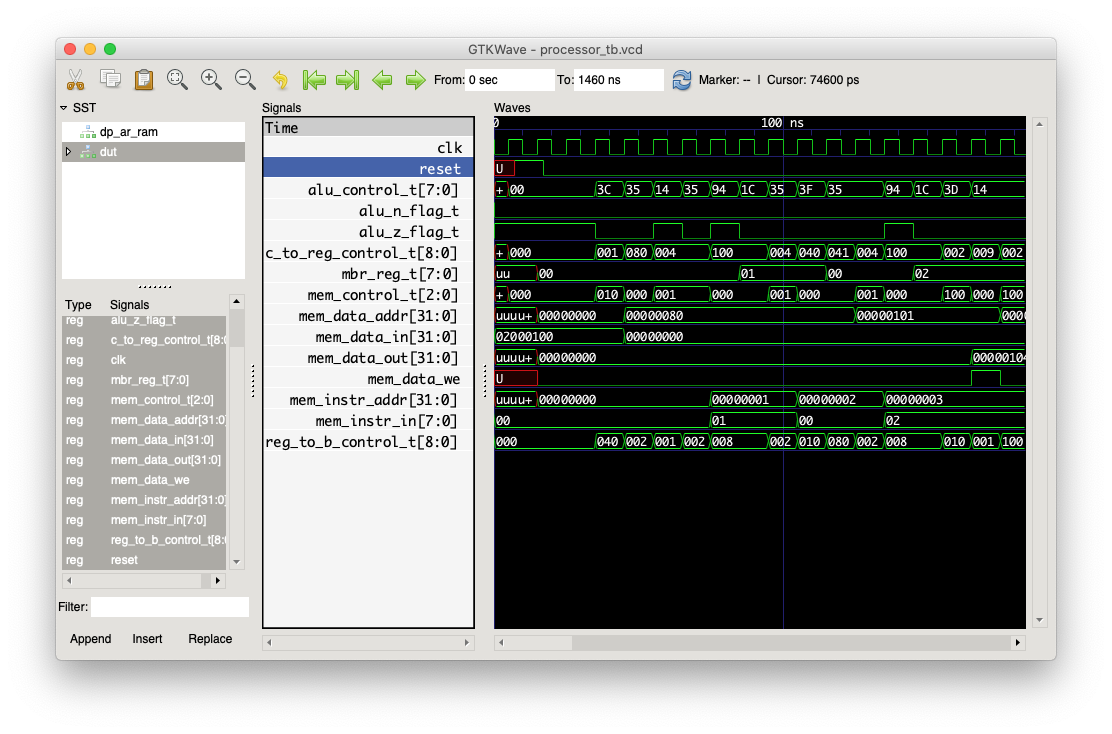
\includegraphics[width=\textwidth]{waveform.png}
  \end{center}
\end{frame}

\section{Tracce}
\begin{frame}
  \frametitle{Tracce degli Esercizi}
  \begin{enumerate}
    \item Simulare l'esecuzione di un programma contenente due istruzioni IJVM.
    \begin{itemize}
      \item È necessario modificare il programma (\lstinline{program.ajvm}) e
      ricreare la RAM.
      \item Dunque, si può aggiungere un nuovo testbench alla suite o
      modificare quello già esistente (\lstinline{processor_tb.vhd}).
    \end{itemize}
    \item Modificare l'operazione eseguita da un'istruzione IJVM.
    \begin{itemize}
      \item È necessario modificare il microprogramma (\lstinline{ajvm.mal}) e
      ricreare il control store.
      \item Che succede modificando la \lstinline{IADD}? Come possiamo farle
      eseguire una sottrazione?
    \end{itemize}
  \end{enumerate}
\end{frame}

\begin{frame}
  \frametitle{Esercizi \textbf{Facoltativi}}
  \begin{enumerate}
    \setcounter{enumi}{2}
    \item Sintetizzare su FPGA il processore.
    \begin{itemize}
      \item Così come implementato, potrebbe essere "troppo grande" per
      alcune board;
      \item in questo caso, conviene ridurre la dimensione della RAM:
      \begin{itemize}
        \item nel file \lstinline{dp_ar_ram.vhd} va ridotta la distanza tra
        l'area codice e il constant pool;
        \item nel file \lstinline{datapath.vhd} va corretto il puntatore al
        constant pool e quello allo stack;
        \item infine, nel file \lstinline{common_defs.vhd} va ridotta la
        dimensione della RAM, impostando \lstinline{dp_ar_ram_size} e.g. a
        64 word da 32 bit.
      \end{itemize}
    \end{itemize}
    \item Collegare al processore una o più periferiche di IO.
    \begin{itemize}
      \item Un esempio completo è fornito nel branch \lstinline{pwm} del
      repository git;
      \item all'instruction set  sono state aggiunte le istruzioni \lstinline{gload} e
      \lstinline{gstore} per interfacciarsi con i registri memory mapped delle
      periferiche;
      \item il file \lstinline{device_mux.vhd} implementa una logica elementare
      per assegnare parte dello spazio di indirizzamento alle periferiche di IO.
    \end{itemize}
  \end{enumerate}
\end{frame}
\end{document}
